\documentclass[11pt,a4paper]{article}
\usepackage{siunitx} % si eenheden
\usepackage{hyperref}					% maak PDF van de thesis navigeerbaar
\usepackage{url}
\usepackage[toc,acronym,xindy]{glossaries}%voor afkortingen
\usepackage{amsmath}
\usepackage[official]{eurosym} % om euro symbool te kunnen gebruiken
\usepackage{graphicx}
\usepackage{svg}
\usepackage[final]{pdfpages}
\usepackage[square,numbers]{natbib} 
\bibliographystyle{IEEEtran}
\usepackage{tabularx}

% =========== BELANGRIJK VR IN HET VERSLAG: Tonen dat je hebt nagedacht over dimensionering componenten! ===========

% MFA: zet zoekpad voor figure
\graphicspath{{fig/}}
\usepackage{float}                      % De optie H voor de plaatsing van figuren op de plaats waar je ze invoegt. bvb. \begin{figure}[H]

\begin{document}
\title{Embedded systems 2\\
	\Huge Report Cosy Cafeteria
}
\author{Robin Van de Poel\and Arthur Van den Storme\and Tobias Cromheecke\and Thomas Feys}
\date{\today}
\maketitle
\newpage

\tableofcontents
\newpage

\section{Intro}
To improve the experience of the students in the cafeteria, an embedded system will be developed to gather a variety of data. This data will then be display to the students through an online medium such as a website. The main focus will be to gather information about the amount off people that are in the cafeteria. There are two main goals. The first goal is to display the estimated waiting time to get a meal to the students. Secondly the amount of available seats will be tracked and displayed to the students. Next to this some additional information will be gathered. The temperature, air-quality and sound level will be monitored to give the student a general idea about the conditions in the cafeteria. This way the student can gauge if the cafeteria is suitable to study in at a certain moment. An overview of the envisioned system is displayed in figure~\ref{fig:system}. All the developed hardware and software is displayed at: \url{https://github.com/thomasf10/cosy_cafeteria}.
\begin{figure}[H]
	\centering
	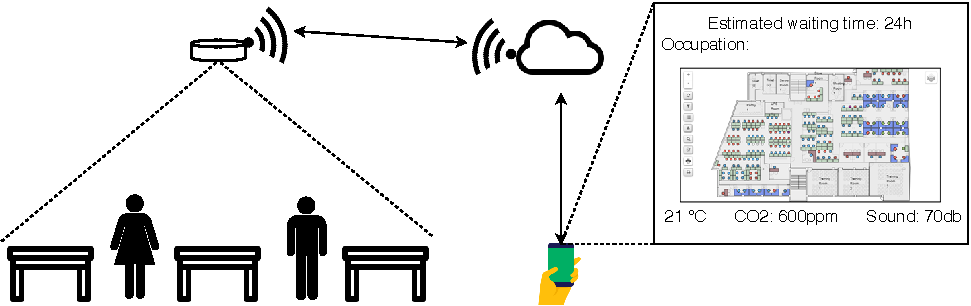
\includegraphics[width=1.0\linewidth]{situation.pdf}
	\caption{Situation sketch}
	\label{fig:system}
\end{figure}

\section{Specifications}
Zoals we geleerd hebben in dit vak? eerst specs opstellen

\section{Functionality}
%- wat gaat uw systeem juist doen

The developed system uses three sensors: 
\begin{itemize}
	\item AMG8833: IR grid sensor
	\item CSS811: air quality sensors
	\item Sparkfun sound detector: microphone
\end{itemize}
By incorporating these sensors in to the system, a variety of sensor data is gathered, namely: ambient temperature [\SI{}{\celsius}], $CO_2$-level [ppm], TVOC-level (total volatile organic compounds) [ppb] and sound level [db]. Next to this the AMG8833 captures the temperature af a two dimensional area in 8 by 8 pixels. 
\\ \\
The 'brain' of the system is an ESP32, this microcontroller has an integrated Wi-Fi module, which will be used to transmit the data. The gathered data is sent to a server, which stores the received data in a database. 
\\ \\
Alongside the reception of data from the ESP32, the server hosts a website which is used to display the data to the students. The website uses the pixel data to generate a heatmap of the cafeteria, this allows the students to see how many people are present in the cafeteria. Unfortunately one module cannot cover the entire cafeteria, to generate the heatmap. In order to do this, several modules have to be deployed in the cafeteria. In this project only one module will be constructed as a proof of concept. Next to the heatmap, the other sensor data is displayed on the website this includes: ambient temperature, $CO_2$-level, TVOC-level and the sound-level. Based on these parameters the students can gauge if the cafeteria is currently suitable as a study-location.

\section{System architecture}
systeem wat uitleggen \dots
\textbf{EENS CHECKEN OF DE ARCHITECTUUR IN GROTE LIJNEN KLOPT}
An overview of the full system is displayed in figure~\ref{fig:architecture}.
\begin{figure}[H]
	\centering
	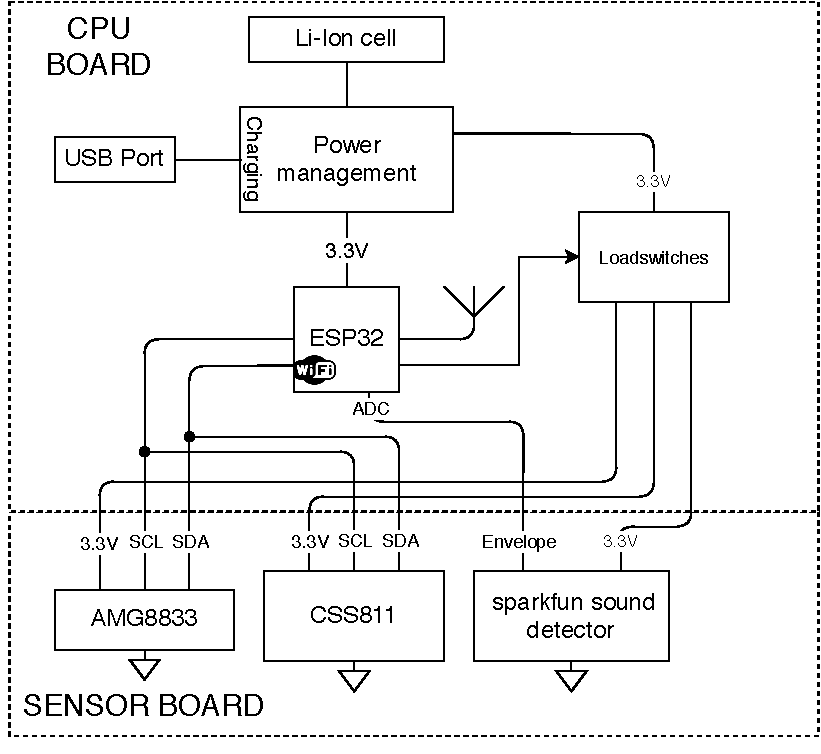
\includegraphics[width=1.0\linewidth]{architecture.pdf}
	\caption{System architecture}
	\label{fig:architecture}
\end{figure}

\section{Power management design}
This section explains the different trade-off's which were made in designing the power management part of the system. The first part in designing the power management is choosing a way to supply the circuit. In our case, the device needs to be deployed at the ceiling of a cafeteria. You can't just tap off the electricity cable at any point here, so our device will need a battery to supply the power. Our first aim was to supply the device as long as one semester. Another aspect was the ability to recharge the battery for environmental reasons. This excludes standard cell batteries that have a much lower energy density and are not rechargeable. Our choice was quickly made for the type of battery, namely a Lithium-Ion (Li-Ion) battery which will be discussed in section \ref{sec:liIon}.

\subsection{Lithium-Ion battery}\label{sec:liIon}
Lithium-Ion batteries are now a commonly used battery in consumer electronics. Li-Ion batteries is the most commonly used battery in phones, MP3 players and other portable equipment. The voltage of a single Li-Ion battery cell is usually fixed at 3.6 V or 3.7 V. We call this the nominal voltage. However, the actual voltage during use can vary from 2.4 V to 4.2 V. When the voltage drops below 2.4 V, the cell is discharged too deeply and damaged beyond repair. Therefore, a safety voltage of 3 V is often maintained. If the cell is discharged to this voltage, nothing is wrong. Charging a Li-Ion battery usually takes 3 hours. Don't be blinded by fast chargers for these batteries, practical tests have shown that it takes 3 hours until a battery is fully charged \cite{LiIon_ledscherp}. A few benefits of a Li-Ion battery are:
\begin{itemize}
	\item Very high energy density
	\item Minor self-discharge
	\item No memory effect
	\item High power, long service life
\end{itemize}
Some disadvantages are:
\begin{itemize}
	\item Relatively expensive to purchase
	\item Dangerous if used incorrectly, can explode/combust
	\item Need a protection circuit to not drop below the 2.4 V threshold value
	\item Charging and discharging process needed 
\end{itemize}
The most common Li-Ion battery is the 18650 cylindrical cell which is 18mm wide, 65mm long and the '0' stands for its cylindrical shape. Another common type of Lithium-Ion battery is the Lithium-Ion Polymer (Li-Po) battery.
%Li-Po's are:
%\begin{itemize}
%	\item Lighter
%	\item Faster recharge
%	\item Higher power: it's easy to produce batteries that can discharge 10C, 20C\footnote{\url{https://batteryuniversity.com/learn/article/what_is_the_c_rate}}.
%	\item Safer: less ability to explode/combust
%	\item Flexible: can bent (up to $90^\circ$) and deform + can be made in a variety of shapes
%	\item More expensive
%\end{itemize}
Li-Po's are preferred over standard Li-Ion batteries in application where weight reduction is important, fast charge opportunity is needed and which need a very high current during discharge time. Li-Po's are more used for drones (where lightweight is a requirement) and electric cars (fast charging requirement). Li-Po's are also less likely to combust or explode and are more expensive. Therefor a Li-Po would be overkill in our application \cite{LiIonVsLi-Po_Ovonic,LiIon_Wiki,Li-Po_Wiki}. 

\subsubsection{Selected battery}\label{sec:selected_battery}
The reason we chose a single cell Li-Ion battery was:
\begin{itemize}
	\item Voltage range: our microcontroller needs 3.3 V supply voltage, which is only a low dropout voltage of 0.4 V in comparison with the 3.7 V nominal voltage of a single cell Li-Ion battery. This results in less power dissipation in the voltage regulator. 
	\item Rechargeable: for environmental aspects
	\item High capacity: around 3000 mAh, to last a semester
\end{itemize}
The specifications of the chosen NCR18650B are:
\begin{itemize}
	\item Size/package: 18650
	\item Rated capacity: 3200 mAh
	\item Nominal voltage: 3.6 V
	\item Maximum voltage: 4.2 V
	\item Maximum charge current: 1625 mA
	\item Maximum discharge current: 6400 mA\footnote{Maximum discharge rate is 2C. This means discharging the battery capacity in 0.5 hours $\frac{3200 mAh}{0.5 h} = 6400 mA$ .} % https://batteryuniversity.com/learn/article/what_is_the_c_rate
	\item Maximum discharge voltage: 2.5 V
	\item Charge time: 4 hours
	\item No protection circuit
\end{itemize}
To charge the Li-Ion we had to include a charge circuit in our design. We found a high frequently used breakout board to charge a single cell Li-Ion battery via USB with battery protection \href{http://acoptex.com/project/9446/basics-project-082a-lithum-battery-charger-tp4056-at-acoptexcom/#sthash.3qJ5RSCy.AsMaJFMH.dpbs}{here}. Such a charge circuit would be perfect for our application. Due the reason we couldn't use a breakout board we had to integrate the components on one PCB. Unfortunately the components which were used on the breakout board were not available on the websites we're using to order components like Mouser, Digi-Key, Farnell, etc. After some research and a recommendation of a fellow student who had experience with battery charging applications in his master thesis, he advised to go for Texas Instruments IC's for charging Li-Ion batteries. The charger IC didn't had a protection circuit on it, so we also needed a circuit for this. Eventually we also went for a protection IC and voltage regulator of Texas Instruments. For reverse polarity of the battery protection we also included an own-designed circuit which was first evaluated in LT Spice. All named components will be discussed in the following sections.

\subsection{Battery charging circuit}

\subsection{Battery protection circuit}
Due the battery we selected doesn't has an integrated protection circuit, we also needed to consider a battery protection circuit in our design. As discussed in section \ref{sec:liIon} it could lead to battery defect when the voltage of the battery drops below 2.4 V threshold value. A Li-Ion is also likely to explode/combust when charging too high in voltage or current. Therefor a protection circuit is always needed. We went for the BQ29700 which is a battery cell protection IC that provides an accurate monitor and trigger threshold for overcurrent protection during high discharge/charge current operation or battery overcharge conditions. The BQ29700 provides the protection functions for Li-Ion/Li-Po cells, and monitors across the external power FETs for protection due to high charge or discharge currents. Figure \ref{fig:bq29700_principeschema} shows the simplified schematic of the BQ29700 IC. In normal mode FETs Charge FET (CHG) and Discharge FET (DSG) are closed, however in one of the following conditions the FETs will open to stop the current flow from/to the battery:
%The system is operating in NORMAL mode when the battery voltage range is between the over-discharge detection threshold (VUVP) and the overcharge detection threshold (VOVP), and the V– pin voltage is within the range for charge overcurrent threshold (VOCC) to over-discharge current threshold (VOCD) when measured with respect to VSS. If these conditions are satisfied, the device turns ON the drive for COUT and DOUT FET control.
\begin{enumerate}
	\item \textbf{Overcharge detection (OVP):} When the cell exceeds the overcharge detection threshold voltage $V_{OVP}$ during charge, the safety circuit will interrupt the flow of current into the cell.% by opening CHG.
	When the overcharge voltage is exceeded, a delay of up to $t_{OVP}$ will occur before the FETs open the circuit.
	\item \textbf{Over-discharge detection (UVP):} When the cell exceeds the over-discharge detection threshold voltage $V_{UVP}$ during discharge, the safety circuit will interrupt the flow of current out of the cell.% by opening DSG. 
	When the over-discharge voltage is reached, a delay $t_{UVP}$ will occur before the FETs open the circuit.
	\item \textbf{Charge overcurrent detection (OCC):} When the pack output current the charge overcurrent detection threshold voltage $V_{OCC}$ during charge, the safety circuit will interrupt the flow of current out of the pack. When the charge overcurrent threshold voltage is exceeded, a delay of up to $t_{OCC}$ will occur before the FETs open the circuit.
	\item \textbf{Discharge overcurrent detection (OCD):} When the pack output current the discharge overcurrent detection threshold voltage $V_{OCD}$ during discharge, the safety circuit will interrupt the flow of current out of the pack. When the discharge overcurrent threshold voltage is exceeded, a delay of up to $t_{OCD}$ will occur before the FETs open the circuit.
	\item \textbf{Load short-circuit detection (SCD):} Similar to overcurrent threshold values, except a short circuit will result in a much higher current, thus a higher sense voltage. The short-circuit detection threshold voltage is indicated as $V_{SCD}$ with delay $t_{SCD}$.
\end{enumerate}
Specifications of the BQ29700 IC are \cite{bib:BQ29700}:
\begin{itemize}
	\item $V_{OVP}$ = 4.275 V
	\item $t_{OVP}$ = 1.25 s
	\item $V_{UVP}$ = 2.8 V
	\item $t_{UVP}$ = 144 ms
	\item $V_{OCC}$ = –0.1 V
	\item $t_{OCC}$ = 8 ms
	\item $V_{OCD}$ = 0.1 V
	\item $t_{OCD}$ = 20 ms
	\item $V_{SCD}$ = 0.5 V
	\item $t_{SCD}$ = 250 $\mu s$
\end{itemize}
\begin{figure}[H]
	\centering
	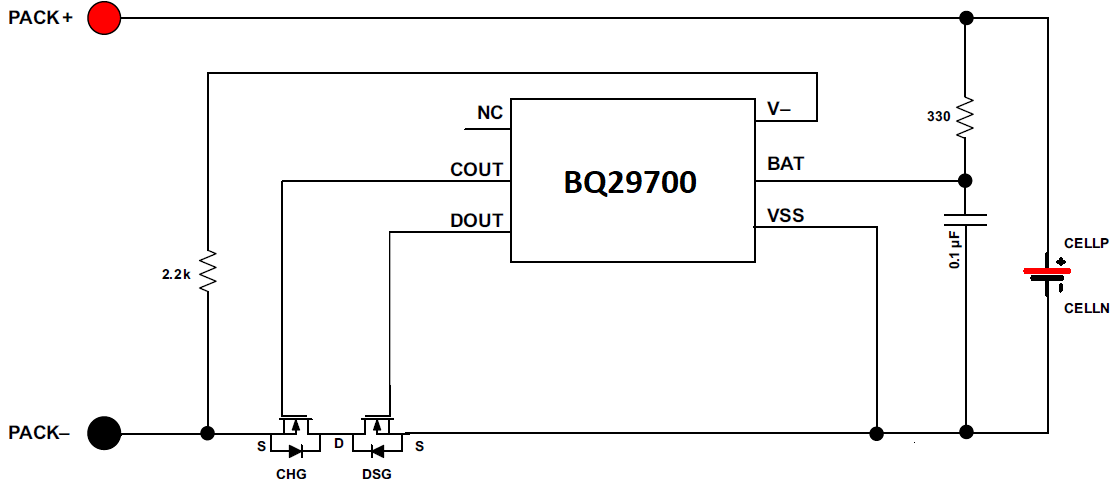
\includegraphics[width=0.9\linewidth]{bq29700_principeschema.png}
	\caption{Simplified schematic BQ29700}
	\label{fig:bq29700_principeschema}
\end{figure}

\subsubsection{Dimensioning}
Figure \ref{fig:bq29700_toegepast} shows the implemented BQ29700 IC in our design. An RC filter is required on the BAT-pin for noise, and enables the device to operate during sharp negative transients. The 330 $\Omega$ resistor also limits the current during a reverse connection on the system. TI recommends placing a high impedance 5 M$\Omega$ across the gate source of each external FET to deplete any charge on the gate-source capacitance. The voltage sense node $V_-$ is a sense node used for measuring several fault detection conditions, such as overcurrent charging or
overcurrent discharging configured as Vds sensing for protection. This input, in conjunction with VSS, forms the differential measurement for the stated fault detection conditions. A 2.2 k$\Omega$ resistor is connected between this input pin and Pack– terminal of the system in the application.
\\ \\
\textbf{FET Selection:} These should be power MOSFETs (range 1-2A, because of limitation of battery charge current of 1625mA and \textbf{!!aanvulle: oplaadstroom USB!!}) who operate at relativly low voltages (2.8-4.2V battery cell). Due the current is measured by the voltage drop across the FETs, it's $R_{DSON}$ value is also an important value by choosing the right MOSFET. We chose FDS9926A, as it's a dual N-channel MOSFET IC. So both charge and discharge MOSFETs are integrated in one IC. Each FET's $R_{DSON}$ = 35 m$\Omega$ at Tj = 25 $^\circ$C and Vgs = 3.7 V (nominal battery voltage) \cite{bib:FDS9926A}. Because both discharge and charge overcurrent detection levels are the same (100 mV), the discharge and charge current are limited to approximately $\frac{100 mV}{2 \cdot 35m\Omega}$ = 1.43 A \cite{bib:BQ29700, bib:FDS9926A}.
\begin{figure}[H]
	\centering
	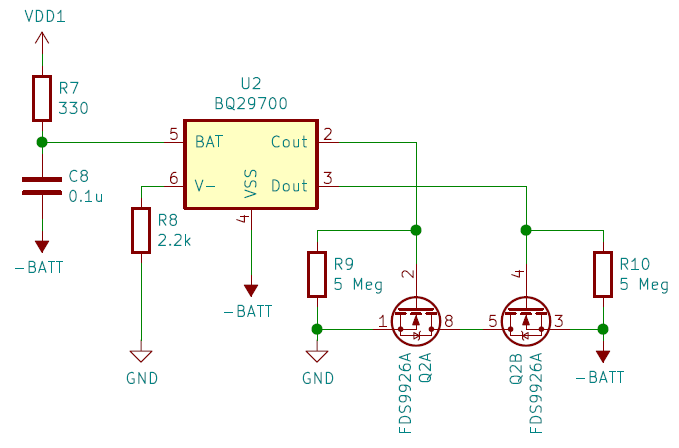
\includegraphics[width=0.9\linewidth]{bq29700_toegepast.png}
	\caption{BQ29700 in our design}  %% AANPASSEN!!!
	\label{fig:bq29700_toegepast}
\end{figure}

\subsection{Reverse polarity protection}
Spice simulaties toevoegen!

\subsection{Voltage regulator}

\section{Microcontroller}

\section{Sensorboard}

% ============ Geofrey wil zien dat we hebben nagedacht over de dimensionering van de componenten !!! ============


\section{Selection battery charger components}
There are many manufacturers who produce charging IC's  bla bla bla ...

We considerd many chips from different kind of manufacturers. Eventualy we went with the BQ24075 IC from Texas Instruments. It's a great chose because it's made to charge a single cell Li-Ion battery (that's all we need), and it's perfectly fit to charge using a USB port because the IC has a selectable 100 mA and 500 mA maximum input current \textbf{TO DO: VERWIJZEN NAAR USB TABEL}. \textbf{OOK NOG ZEGGEN DAT DE OPLAADSTROOM OVEREENKOMT MET DIE VAN DE BATTERY}. In the subsections below you'll find the calculations.

\subsection{Charging}
Set $\overline{CE}$ low to initiate battery charging. The battery is charged in three phases: 
\begin{enumerate}
	\item Conditioning pre-charge
	\item Constant current fast charge (current regulation) 
	\item Constant voltage tapering (voltage regulation)
\end{enumerate}
\begin{figure}[H]
	\centering
	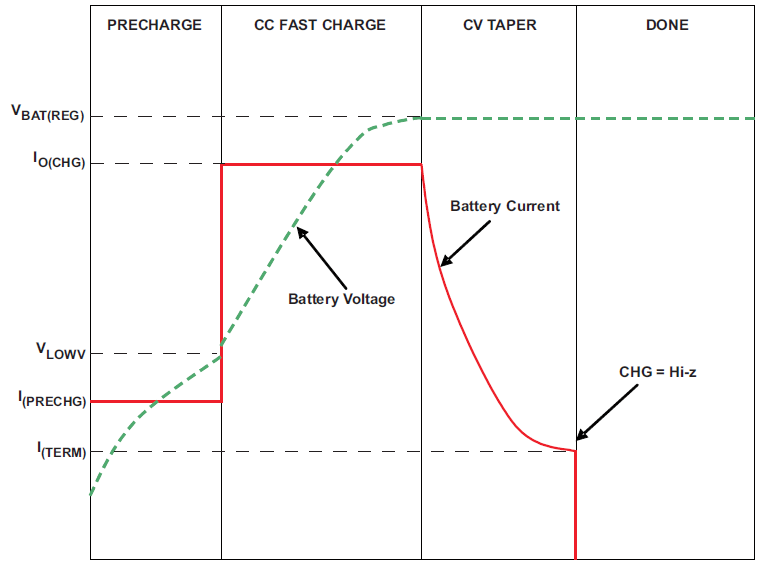
\includegraphics[width=1.0\linewidth]{Charge_cycle}
	\caption{Charge cycle}
	\label{fig:Charge _cycle}
\end{figure}
In the pre-charge phase, the battery is charged at with the pre-charge current $I_{PRECHG}$. Once the battery voltage crosses the $V_{LOWV}$ threshold, the battery is charged with the fast-charge current $I_{CHG}$. As the battery voltage reaches $V_{BAT(REG)}$, the battery is held at a constant voltage of $V_{BAT(REG)}$ and the charge current tapers off as the battery approaches full charge. When the battery current reaches $I_{TERM}$, the CHG pin indicates charging done by going high-impedance.

The value of the fast-charge current is set by the resistor connected from the ISET pin to VSS, and is given by the equation:
\[ I_{CHG} = \frac{K_{ISET}}{R_{ISET}} \]
The charge current limit is adjustable up to 1.5 A. The valid resistor range is 590 $\Omega$ to 8.9 k$\Omega$. If $I_{CHG}$ is programmed as greater than the input current limit, the battery will not charge at the rate of $I_{CHG}$, but at the slower rate of $I_{IN(MAX)}$ (minus the load current on the OUT pin, if any). In this case, the charger timers will be proportionately slowed down.

\subsubsection{Charge Current Translator}
When the charger is enabled, internal circuits generate a current proportional to the charge current at the ISET input. The current out of $I_{SET}$ is 1/400 ($\pm$10\%) of the charge current. This current, when applied to the external charge current programming resistor, $R_{ISET}$, generates an analog voltage that can be monitored by an external host to calculate the current sourced from BAT.
\[ V_{ISET} = \frac{I_{CHG}}{400} R_{ISET} \]

\subsection{System enable input}
Connect SYSOFF high to turn off the FET connecting the battery to the system output. When an adapter is connected, charging is also disabled. Connect SYSOFF low for normal operation. SYSOFF is internally pulled up to VBAT through a large resistor (approximately 5 M$\Omega$). Do not leave SYSOFF unconnected to ensure proper operation.

\subsection{Calculations}
\subsubsection{Program the Fast Charge Current $I_{CHG}$}
\[ R_{ISET} = \frac{K_{ISET}}{I_{CHG}} \]
From the electrical table we can find:
\[ K_{ISET} = 890 A\Omega \]
The charge current limit is adjustable up to 1.5 A. The maximum charge current for the Panasonic NCR18650B battery is 1625 mA. Set the charge current to 1.3 A to have some margin for the battery lifetime.
\[ R_{ILIM} = \frac{890 A\Omega}{1.3 A} = 684.62 \Omega \approx 680 \Omega \]
The valid resistor range is 590 $\Omega$ to 8.9 k$\Omega$. Select the closest standard value, which for this case is 680 $\Omega$. Connect this resistor between ISET (pin 16) and VSS.
\[ I_{CHG} = \frac{890 A\Omega}{680 \Omega} = 1.31 A \]

\subsubsection{Program the Input Current Limit $I_{LIM}$}
\[ R_{ILIM} = \frac{K_{ILIM}}{I_{IN(MAX)}} \]
From the electrical table we can find:
\[ K_{ILIM} = 1610 A\Omega \]
The input current limit is adjustable up to 1.5 A. Set the input current limit higher than the charge current of 1.3 A.
\[ R_{ILIM} = \frac{1610 A\Omega}{1.5 A} = 1.073 k\Omega \approx 1.1 k\Omega  \]
The valid resistor range is 1.1 k$\Omega$ to 8 k$\Omega$. Select the closest standard value, which for this case is 1.1 k$\Omega$. Connect this resistor between ILIM (pin 12) and VSS.
\[ I_{ILIM} = \frac{1610 A\Omega}{1.1 k\Omega} = 1.46 A \]

\subsubsection{Fast-Charge Safety Timer (TMR)}
Leave TMR open to set to default safety timers. Connect to VSS to disable safety timers.

\subsubsection{TS function}
Connect a 10 k$\Omega$ resistor from TS to VSS to set the TS voltage at a valid level and maintain charging.

\subsubsection{Selecting IN, OUT, and BAT Pin Capacitors}
In most applications, all that is needed is a high-frequency decoupling capacitor (ceramic) on the power pin, input, output and battery pins. Using the values shown on the application diagram, is recommended. After evaluation of these voltage signals with real system operational conditions, one can determine if capacitance values can be adjusted toward the minimum recommended values (DC load application) or higher values for fast high amplitude pulsed load applications. Note if designed high input voltage sources (bad adaptors or wrong adaptors), the capacitor needs to be rated appropriately. Ceramic capacitors are tested to 2x their rated values so a 16-V capacitor may be adequate for a 30-V transient (verify tested rating with capacitor manufacturer).

\subsubsection{Selecting MOSFETs}
Discharge Overcurrent Detection (OCD) voltage = 100 mV. $R_{DSON} = 30 m\Omega @ V_{GS} = 4.5 V$
Maximum operating discharge current = $\frac{100 mV}{2 \cdot 30 m\Omega} = 1.67 A$

\section{Wireless connectivity}
\subsection{Wi-Fi connection}
In order to transmit the sensor data to the server, the Wi-Fi connectivity of the ESP32 is used. The transmission is provided by a TCP connection that is established between the ESP32 and the python server. At the initialisation of the python server, a socket is opened, this socket is used to receive the data. In this manner, the server is always listening on the socket, until a message is received. The ESP32 sends the data in the following order: pixeldata (64 floats), temperature (1 float), audio level (1 float), $CO_2$-level (1 unint16) and TVOC-level (1 unint64). The received data is processed by order to determine which data is represented by the received values. The data is parsed into different variable, these variables are then used to update the values in the database. 

\subsection{Power consumption}
To determine the power that is consumed when the sensor data is transmitted once, a measurement is performed. The current consumption is measured, the result is displayed in figure~\ref{fig:wifi_pwr}.
\begin{figure}[H]
	\centering
	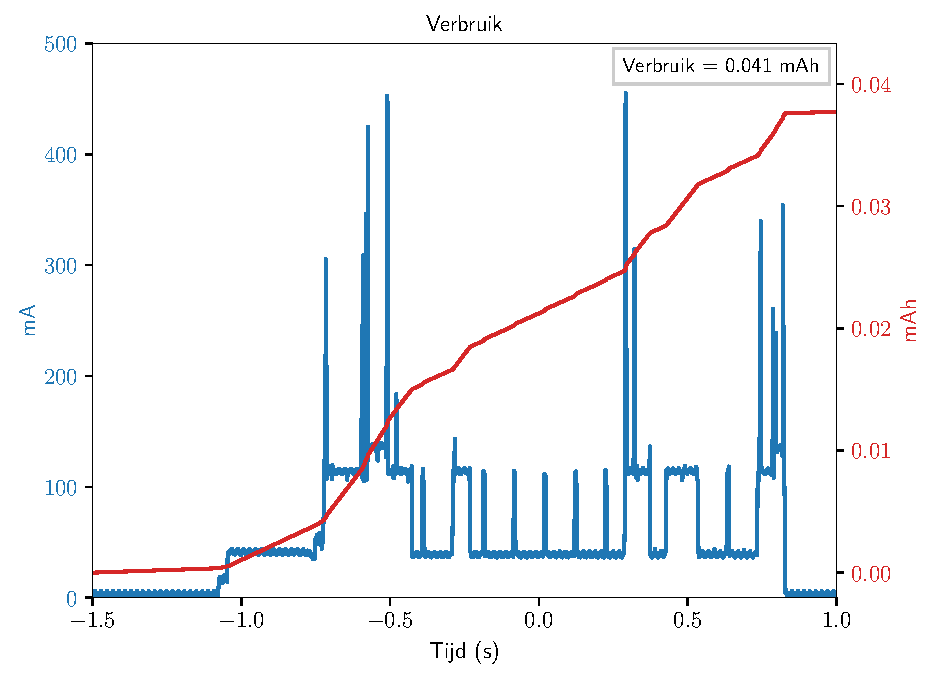
\includegraphics[width=1.0\linewidth]{wifi_pwr.pdf}
	\caption{Power consumption of one Wi-Fi transmission}
	\label{fig:wifi_pwr}
\end{figure}
In order to interpret the current consumption, the used capacity is displayed in [mAh]. This results in 0.041 mAh of capacity that is used in order to transmit the sensor data once. With this knowledge, we can calculate the amount of Wi-Fi transmissions that are possible with the 6400 mAh battery:

\begin{gather*}
	\frac{6400}{0.041} \approx 156097
\end{gather*}

156097 transmissions are possible, if there are 6 transmissions per hour and the system is active for 7 hours a day, this leads to a battery life off 3716 days.  However, this calculation only accounts for the Wi-Fi transmission other power consumption such as stand-by power, CPU power and sensor power are not accounted for in the calculation. 

\section{Software design}
\textbf{todo}
\begin{figure}[H]
	\centering
	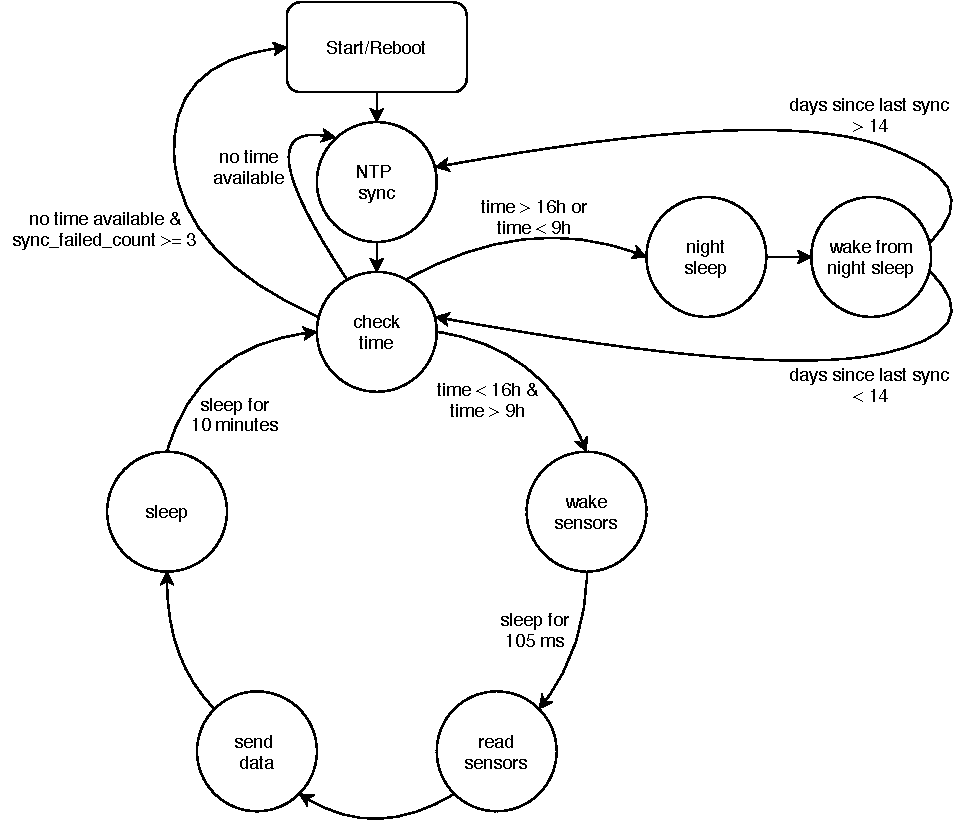
\includegraphics[width=0.8\linewidth]{statendiagram.pdf}
	\caption{State diagram}
	\label{fig:statediagram}
\end{figure}

\section{Autonomy}
Calculations for lifetime.

\section{Website}

\section{Financial estimate}
Kostprijs van het project opstellen.

\section{Validation and measurements}
Hier moeten we aantonen of dat alles werkt. Of eventuele fouten verklaren.

% bibliografie toevoegen
\newpage
\bibliography{bibliography}	

%----------------------------------------------------------------------------------------
%	Bijlagen
%----------------------------------------------------------------------------------------
\newpage
\appendix
\section{MainPCB schematic}\label{app:mainpcb_schematic}
%\begin{figure}[H]
%	\centering
%	\includegraphics[width=1\linewidth]{MainPCB_schematic.pdf}
%\end{figure}
\includepdf{fig/MainPCB_schematic.pdf}

\newpage

\end{document}